% Copyright (c) 2021 Matthew Riehl

% All graphics and documentation in this project are licensed under
% Creative Commons Attribution-ShareALike 3.0 Unported.
% See http://creativecommons.org/licenses/by-sa/3.0/ for the full description.
%
% ALSO:
%
% THE SOFTWARE IS PROVIDED "AS IS", WITHOUT WARRANTY OF ANY KIND, EXPRESS OR
% IMPLIED, INCLUDING BUT NOT LIMITED TO THE WARRANTIES OF MERCHANTABILITY,
% FITNESS FOR A PARTICULAR PURPOSE AND NONINFRINGEMENT. IN NO EVENT SHALL THE
% AUTHORS OR COPYRIGHT HOLDERS BE LIABLE FOR ANY CLAIM, DAMAGES OR OTHER
% LIABILITY, WHETHER IN AN ACTION OF CONTRACT, TORT OR OTHERWISE, ARISING FROM,
% OUT OF OR IN CONNECTION WITH THE SOFTWARE OR THE USE OR OTHER DEALINGS IN THE
% SOFTWARE.

\documentclass[]{article}
\usepackage[table, dvipsnames]{xcolor}% http://ctan.org/pkg/xcolor
\usepackage{fullpage} % Package to use full page
\usepackage{parskip} % Package to tweak paragraph skipping
\usepackage{tikz} % Package for drawing
\usepackage{amsmath}
\usepackage{hyperref}

\title{An Adafruit Metro Express Ohm Meter}
\author{Dr. Matthew Riehl}
\date \today

\begin{document}
\newcommand{\ds}{\displaystyle}
	\maketitle
	\newcommand{\tc}{\textcolor}
	\section{Introduction}
	
	This week, you will build an ohmmeter ($\Omega$-meter) to measure the resistance of individual resistors and combinations of resisters.  The lab can be open-ended and you are encouraged to find ways to improve the circuit and code to make a more versatile instrument.
	
	\section{Materials}
	The materials below were assembled last time to display a brief message from the Arduino on the LCD.  Check to ensure that the board is still assembled and that the display still works.  If it does not, your first job is to fix it.
	\begin{itemize}
		\item PC with Mu IDE installed.
		\item Adafruit Metro Express board and power cable
		\item Half-size breadboard
		\item LCD display module
		\item 220 $\Omega$ resistor ($\Omega$ is Ohm)
		\item 10 k$\Omega$ potentiometer
		\item Jumper wires
	\end{itemize}
	The materials here are the new parts needed for completion of this weeks project.
	\begin{itemize}
		\item Jumper wires
		\item Resistors (variety)
		\item Commercial multi-meter
	\end{itemize}

	\section{Background}
	Resistors are used control the current and voltage that flows through a circuit and are commercially available with resistances from a few ohms to gigaohms ($1\times 10^9\ \Omega$).  They are also manufactured to tolerances from $\pm 0.05 \%$ to $\pm 10 \% $ because, when choosing a resistor for a circuit, sometimes `close is good enough' and at other times the exact resistance must be known.  Most of the resistors you will encounter have a stated resistance of $\pm 5\%$, so the error is considerable.  If you need to know the resistance in a circuit or through a collection of resistors, an ohmmeter is a useful tool to have in your shop.

	\begin{figure}%[h]
		\centering
		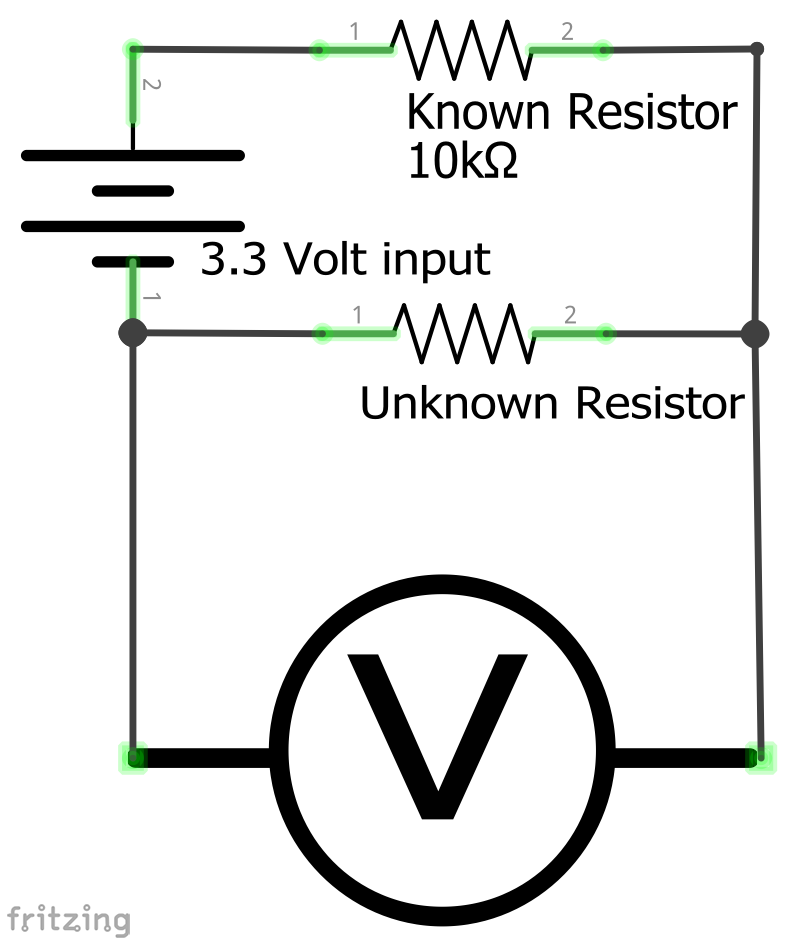
\includegraphics[width=4cm]{pics/voltagedivider.png}
		\caption{Voltage Divider}
		\label{divider}
	\end{figure}

	The ohmmeter works by building a `voltage divider' circuit as shown in Figure \ref{divider}.  The voltage measured by the voltmeter can be calculated as follows:  The battery supplies  some amount of current that passes first through Resistor 1 and then Resistor 2.  Keeping in mind Ohm's law: $\ds V=IR$, we can see that if the current through both resistors is the same (as it must be), then,

	\begin{equation}
		I = \frac{V}{R} = \frac{V_{Resistor\ 1}}{R_{Resistor\ 1}} = \frac{V_{Resistor\ 2}}{R_{Resistor\ 2}} 
	\end{equation}

	Recall that $\ds V = \frac{EPE}{q}$ and the electrical potential energy is consumed, or lost, as the charges flow through the circuit.  There is a voltage drop through each leg of the circuit (through each resistor) which can be measured with a voltmeter. If the voltage supplied to the circuit by the battery is 3.3 V, the  measured voltage (the drop across Resistor 2) will always be less than 3.3 volts, but how much less depends on the resistances of both resistors.  In the simple case where $R_1 = R_2$, the voltmeter will read 2.5 Volts, but as $R_2$ becomes smaller, the voltage drop across \(R_2\) becomes larger.  From this observation and Ohm's law, we conclude that a smaller resistance in a circuit allows more current to flow. 

  	For the circuit shown in Figure \ref{divider}, we can write:
	\begin{equation}
		V= V_1 + V_2 = IR_1 + IR_2 = I(R_1 +R_2) = IR_{equivalent}
	\end{equation}
	where $R_{equivalent}$ is the sum of the resistors or the equivalent resistance.  Since the current is the same through each leg of the circuit, we can make the substitution $\ds I = \frac{V_2}{R_2}$ and rearrange:
	\begin{equation}
		V=\frac{V_2}{R_2}(R_1 +R_2)
		\label{voltage}
	\end{equation}
	\begin{equation}
		V_2=\left(\frac{V}{R_1+R_2}\right)R_2
		\label{VDiv}
	\end{equation}

	Equation \ref{VDiv} is the general equation for a voltage divider.  A power source may supply more voltage than is needed for a particular application and the voltage can be reduced by choosing a combination of resistors such that $V_2$ is the desired voltage.

	For our purposes today, however, we will measure $V_2$ and use our knowledge of V and $R_1$ to determine the value of $R_2$.  Equation \ref{voltage} can be rearranged to yield

	\begin{equation}
		R_2 = \frac{R_1V_2}{V-V_2}
	\end{equation}

	and this is the equation we will program into the micro-controller.

\section{Metro Express Wiring}

	The LCD display you built last time will not be changed.  You will add a few wires and one resistor to the breadboard to complete the voltage divider circuit.  The 3.3 volts potential will be supplied by the Adafruit 3.3\,V pin\footnote{The Adafruit Digital-Analog Converter (DAC) works with the 3.3 volt power.  It cannot be used with 5 volts like the Arduino.}. The circuit will be completed by connecting the voltage divider to the ground in the power strip.  A resistor of known resistance  will be added to the circuit as shown. Two leads may be used to connect to the unknown resistor or resistors if desired.  The green wire is used to measure the voltage between $R_2$ and the ground, and it is connected to the A5 pin on the Metro Express.  The A0 - A5 pins on the Adafruit are analog pins.  The Arduino then digitizes the voltage -- it assigns a digital value where 0 equals 0 volts and 65536 equals 3.3 volts (\(65536=2^{16}\)); you will see in the code that the value taken from A5 must be multiplied by $\frac{3.3}{65536}$ to yield a voltage.

% see http://www.circuitbasics.com/arduino-ohm-meter/ for more information.
	\begin{figure}[h]
		\centering
		\begin{tikzpicture}%[scale=0.85]
			\node[anchor=south west,inner sep=0] (image) at (0,0) {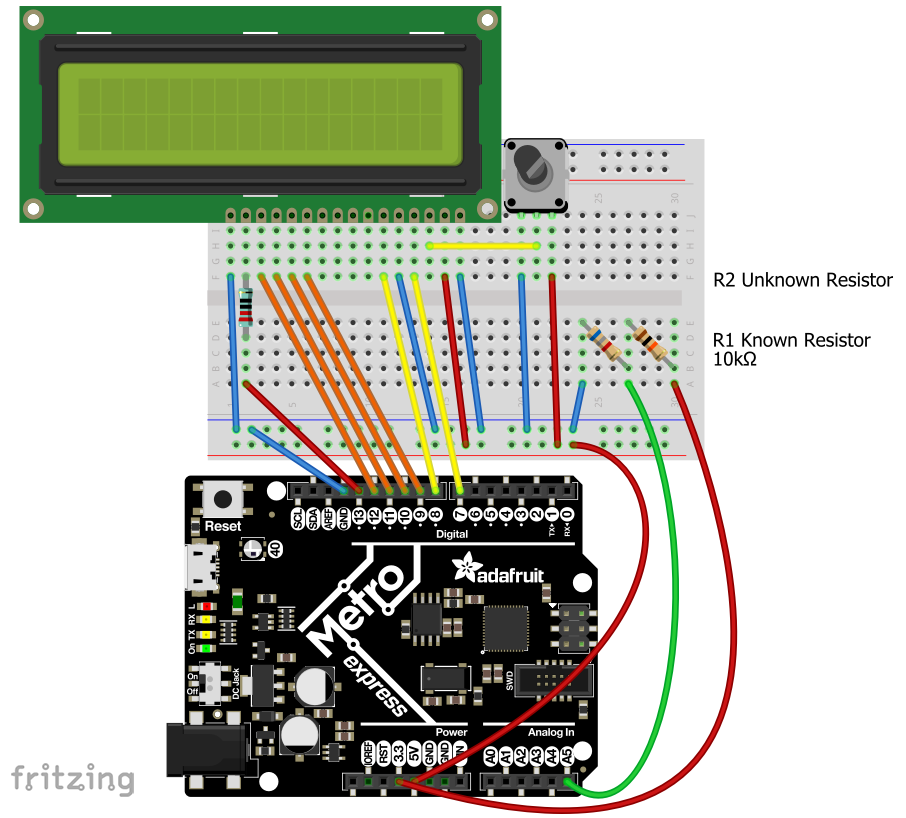
\includegraphics[width=0.75\textwidth]{pics/ohmwiremetro}};
			\node [anchor=west] (ref) at (10.7,5.2) {\small 3.3 Volts};
			%%%% Arrow placement %%%%
			\draw[-latex, red, ultra thick] (9.7,7.4) to[out=180, in=60] (8.15,6.83);
			\draw[-latex, red, ultra thick] (9.7,6.5) -- (9.15,6.5);
			\draw[-latex, red, ultra thick] (10.7,5.2) to[out=180, in=0] (9.8,4.8);
		\end{tikzpicture}
		\caption{Pin-out Diagram for the Adafruit Metro Express Ohmmeter.}
		\label{AdafruitPinOut}
	\end{figure}
	


	The unknown resistors can be added to the circuit as convenient -- the resistor may be connected directly to the breadboard or a second breadboard may be used.  

	\section{Python Code for the Metro Express}

	The code for this weeks lab is reproduced below, but is also included in a separate .py file.  Note that the value of the known resistor is set to $10,000\ \Omega$ in this code (R1=10000;).  You will change this to whatever known resistor you are using.  Remember that you must upload the new code to the Metro Express before it takes effect.

	As supplied, the code will inform you of the resistance coded in for the known resistor and then display the resistance measured for the unknown resistor and the voltage drop across the unknown resistor.  If either resistor is absent or poorly matched to the other resistor (resulting in a large error in the calculated resistance), a message is sent to the LCD and then the display shuts off until the error is fixed.  

	Also note that in the code below, each line is left-justified.  Python requires that the code be indented to indicate flow control.  If you paste the code into the Mu IDE without proper indentations, it will complain.
\begin{verbatim}
"""
This code is included with the files for Adafruit Labs Ohmmeter by
Matthew Riehl and is in the public domain.  I have only modified the
code to better support the laboratory exercise.

Demonstrates the use a 16x2 LCD display.  The LiquidCrystal
library works with all LCD displays that are compatible with the
Hitachi HD44780 driver. There are many of them out there, and you
can usually tell them by the 16-pin interface.

The Ohmmeter circuit uses a voltage divider.  A 3.3 volt potential flows
through two resistors in series.  The first resistor has a known resistance
and is assigned R1 in the code.  (You MUST change R1 in the code to match the 
resistance being used.)  The resistance of the second (unknown) resistor
is calculated from Equation 5 in the handout.  The LCD displays the voltage
drop across R2 (the unknown resististance) and the calculated resistance.  
The accuracy of the measurement drops at voltages approaching 0 (unknown
resistors with resistances much higher than R1) and at voltages approaching
5 volts (unknown resistors with resistances much lower than R1).

If either R1 or R2 are absent or out of range, the display shuts off.

"""
import time
import board
import digitalio
import adafruit_character_lcd.character_lcd as characterlcd
from analogio import AnalogIn

# Define variables and constants
Vin = 3.3
Vout = 0
R1 = 10000  # This is the known resistor -- this value must be
            # changed to the actual value of R1.
R2 = 0
a2d_data = AnalogIn(board.A5)  # Analog to Digital data -- read at A0
buffer = 0
VR2 = 0

def get_voltage(pin):       # A helper program to calculate the voltage at A5
	return ((pin.value / 65536) * 3.3) 

# Modify this if you have a different sized character LCD
lcd_columns = 16
lcd_rows = 2

# Metro M0/M4 Pin Config:
lcd_rs = digitalio.DigitalInOut(board.D7)
lcd_en = digitalio.DigitalInOut(board.D8)
lcd_d7 = digitalio.DigitalInOut(board.D12)
lcd_d6 = digitalio.DigitalInOut(board.D11)
lcd_d5 = digitalio.DigitalInOut(board.D10)
lcd_d4 = digitalio.DigitalInOut(board.D9)
lcd_backlight = digitalio.DigitalInOut(board.D13)

# Initialise the LCD class
lcd = characterlcd.Character_LCD_Mono(
lcd_rs, lcd_en, lcd_d4, lcd_d5, lcd_d6, lcd_d7, lcd_columns, lcd_rows, lcd_backlight
)

lcd.clear()
lcd.backlight = True
lcd.message = "Ohmmeter!"  
time.sleep(3)
lcd.message = ("R1 Resistance \n{}  Ohms ".format(int(R1)))
time.sleep(3)
lcd.clear()

while True:  # This loop continues forever.
	lcd.backlight = True
	buffer = get_voltage(a2d_data)
	lcd.clear()
	if buffer > 0.33 and buffer < 2.97:
		buffer = get_voltage(a2d_data)
		R2 = int(R1 * buffer / (Vin-get_voltage(a2d_data)))
		lcd.message = ("R2 = {} Ohms.".format(R2))
		VR2 = 3.3 - buffer
		VR2 = str(round(VR2, 3))
		lcd.message = ("\nR2 drop {} V.".format(VR2))
		time.sleep(1)
	elif buffer <= 0.33:
		lcd.message = "R1 missing  \n or R1 >> R2."
		time.sleep(4)
		while buffer <= 0.33:
			buffer = get_voltage(a2d_data)
			lcd.clear()
			lcd.backlight = False
	else:
		lcd.message = "R2 missing  \n or R2 >> R1."
		time.sleep(4)
		while buffer >= 2.97:
			buffer = get_voltage(a2d_data)
			lcd.clear()
			lcd.backlight = False

\end{verbatim}

When you have a working ohmmeter, ask your lab instructor for permission before continuing.





	\section{Errors in Measuring Resistance}

	Keep a record of your work and calculations on a separate page that can be turned in with your report.
	\begin{enumerate}
		\item Select a resistor to be your known resistor $R_1$ and insert it into the circuit as shown in the pinout diagram (Figure \ref{AdafruitPinOut}).  Change the value of R1 in the Python code to the resistance of $R_1$ and upload this to the Metro Express.  Be sure to record the value of R1 in your notes.  You may wish to verify the resistance of $R_1$ with a commercial ohmmeter.
		\item Select a variety of resistors  (at least five) to be R2 and use the ohmmeter to measure the resistance across each one.  For each resistor, record the resistance as indicated by the colored bands and record the resistance as determined by your ohmmeter.
		\item Calculate the percent error between the two resistance values.
		\begin{equation}
			\% \ Error = \frac{\text{Expected Resistance - Measured Resistance}}{\text{Expected  Resistance}} \times 100
		\end{equation}
		\item Repeat steps 1 - 3 with a different $R_1$.  Choose resistors for $R_1$ that differ by  orders of magnitude, such as $100\ \Omega$, $1000\ \Omega$, and $100,000\ \Omega$.
	\end{enumerate}

	You should find that the errors are smaller when $R_2$ has about the same resistance as $R_1$.  If this is not the case, inform the lab instructor.
	\newpage
	\section{Resistors in Series and in Parallel}
	Again, please keep a record of your work and calculations on a separate page.

	In this section, you will investigate the resistance of a circuit that contains multiple resistors in series or in parallel.  The Metro Express will measure the resistance of the circuit and you will compare this to the expected resistance of the circuit, calculated from the known resistances of each resistor.

	As we saw earlier, the equivalent resistance of two or more resistors in series is the sum of the individual resistances.
	\begin{equation}
		R_{series} = R_1 + R_2 +\dots = \sum_i R_i
	\end{equation}
	
	When resistors are in parallel, however, the current is divided between the resistors with the smallest resistor receiving the greatest current (the path of least resistance).  It will be shown in class that the equivalent resistance of resistors in parallel is:
	\begin{equation}
		\frac{1}{R_{parallel}} = \frac{1}{R_1} + \frac{1}{R_2} + \dots = \sum_1 \frac{1}{R_i}
	\end{equation}
	
	\begin{enumerate}
		\item Construct circuits that contain at least two or three resistors in series (Figure \ref{seriescircuit}) and measure the resistance with your ohmmeter.  If necessary, replace your $R_1$ with a resistor suitable for the resistance you are measuring.
	
		\item Draw each circuit, label each resistor with the known resistance, and calculated the expected resistance of the circuit.
		\begin{figure}[h]
		\centering
		\begin{tikzpicture}%[scale=0.85]
			\node[anchor=south west,inner sep=0] (image) at (0,0) 	{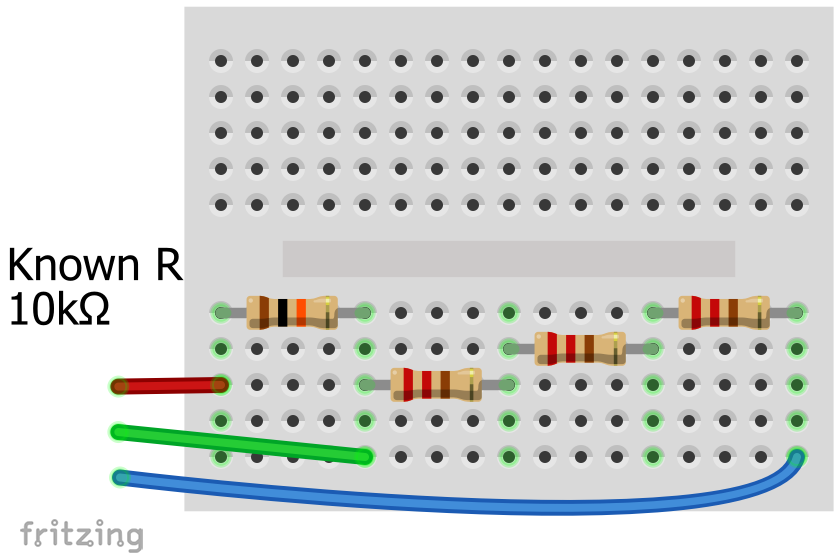
\includegraphics[width=0.5\textwidth]{pics/scircuitbb}};
			\node [anchor=east] (ref) at (0.95,1.7) {3.3 Volt};
			\node [anchor=east] (ref) at (0.95,1.22) {Voltmeter (A5)};
			\node [anchor=east] (ref) at (0.95,.75) {Ground};
			%%%% Arrow placement %%%%
			\draw[-latex, red, ultra thick] (1.8,3) to[out=0, in=120] (2.85,2.68);
		\end{tikzpicture}
		\caption{Three resistors in series circuit diagram}
		\label{seriescircuit}
	\end{figure}
		\item Calculate the percent error.
		\item Repeat steps 1-3 with circuits that contain at least two or three resistors in parallel (Figure \ref{parallelcircuit}).
	
	\begin{figure}
	\centering
	\begin{tikzpicture}%[scale=0.85]
		\node[anchor=south west,inner sep=0] (image) at (0,0) {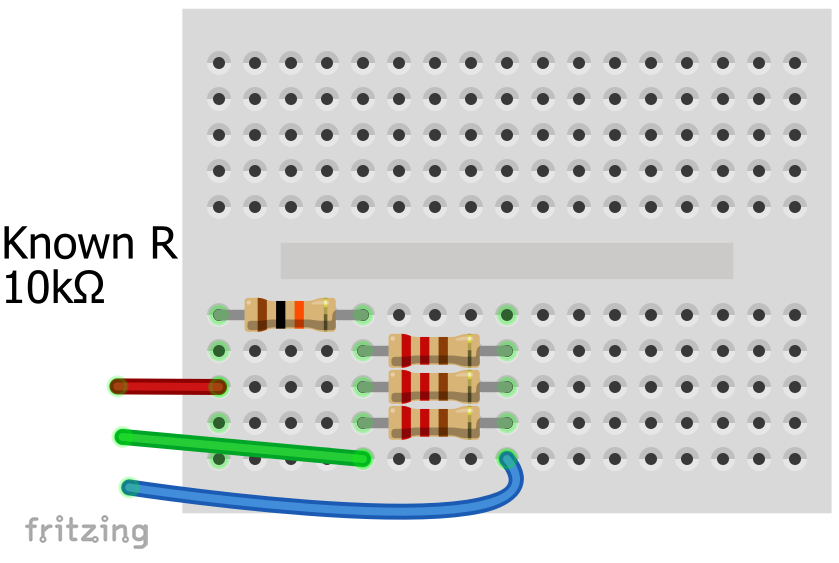
\includegraphics[width=0.5\textwidth]{pics/pcircuitbb}};
		\node [anchor=east] (ref) at (0.95,1.7) {3.3 Volt};
		\node [anchor=east] (ref) at (0.95,1.22) {Voltmeter (A5)};
		\node [anchor=east] (ref) at (0.95,.75) {Ground};
		%%%% Arrow placement %%%%
		\draw[-latex, red, ultra thick] (1.8,3) to[out=0, in=120] (2.85,2.68);
		
		
	\end{tikzpicture}
	\caption{Three resistors in parallel circuit diagram}
	\label{parallelcircuit}
	\end{figure}
	
	
	\item Repeat steps 1-3 with circuits that contain at least three or four resistors with both parallel and series components (Figure \ref{spcircuit}).
	\begin{figure}
	\centering
	\begin{tikzpicture}%[scale=0.85]
		\node[anchor=south west,inner sep=0] (image) at (0,0) {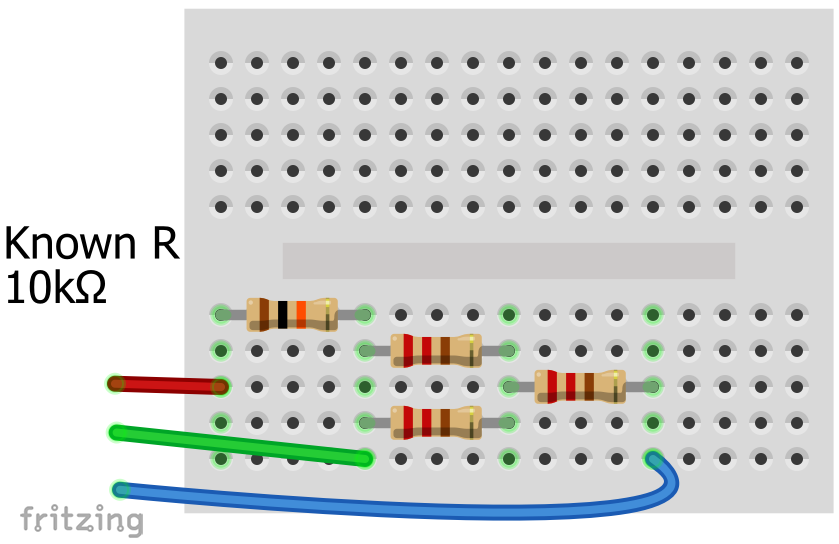
\includegraphics[width=0.5\textwidth]{pics/spcircuitbb}};
		\node [anchor=east] (ref) at (0.95,1.65) {3.3 Volt};
		\node [anchor=east] (ref) at (0.95,1.12) {Voltmeter (A5)};
		\node [anchor=east] (ref) at (0.95,.6) {Ground};
		%%%% Arrow placement %%%%
		\draw[-latex, red, ultra thick] (1.8,3) to[out=0, in=120] (2.85,2.68);
	\end{tikzpicture}
	\caption{Two resistors in parallel, in series with a third}
	\label{spcircuit}
	\end{figure}

	
	\end{enumerate}

	\pagebreak
	\section{Prelab}

	Part 1: Below, you will find thirteen resistors of varying values (Figure \ref{resistors}).  Use the resistor color chart to determine the ohm value of each resistor.  

	\begin{figure}[h]
	\centering
	\begin{tikzpicture}[scale=0.75]
		\node[anchor=south west,inner sep=0] (image) at (0,0) {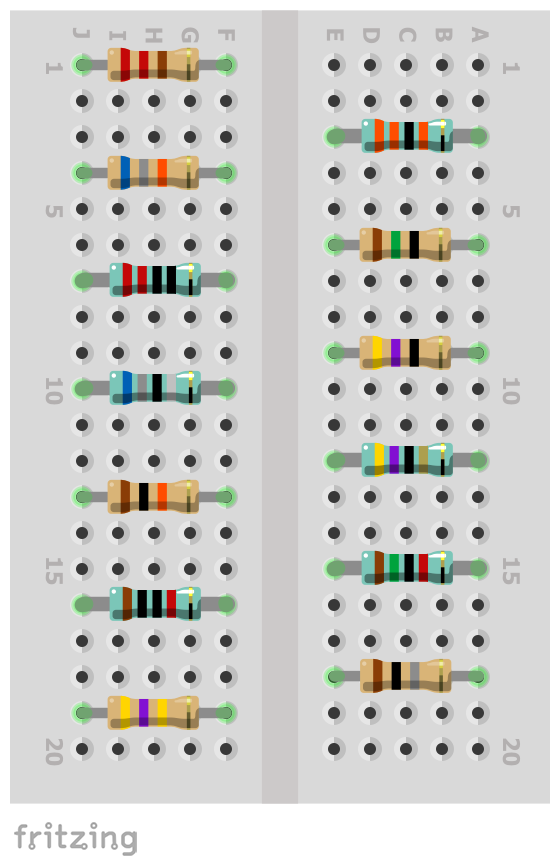
\includegraphics[width=0.5625\textwidth]{pics/prelab}};
		\node [anchor=east] (No1) at (0.0,17.6) {1. \underline{\phantom{blahblah}}};
		\node [anchor=east] (No2) at (0.0,15.21) {2. \underline{\phantom{blahblah}}};
		\node [anchor=east] (No3) at (0.0,12.82) {3. \underline{\phantom{blahblah}}};
		\node [anchor=east] (No4) at (0.0,10.43) {4. \underline{\phantom{blahblah}}};
		\node [anchor=east] (No5) at (0.0,8.036) {5. \underline{\phantom{blahblah}}};
		\node [anchor=east] (No6) at (0.0,5.645) {6. \underline{\phantom{blahblah}}};
		\node [anchor=east] (No7) at (0.0,3.25) {7. \underline{\phantom{blahblah}}};
		%
		\node [anchor=west] (No8) at (12.5,16.1) {8. \underline{\phantom{blahblah}}};
		\node [anchor=west] (No9) at (12.5,13.7) {9. \underline{\phantom{blahblah}}};
		\node [anchor=west] (No10) at (12.5,11.3) {10. \underline{\phantom{blahblah}}};
		\node [anchor=west] (No11) at (12.5,8.9) {11. \underline{\phantom{blahblah}}};
		\node [anchor=west] (No12) at (12.5,6.5) {12. \underline{\phantom{blahblah}}};
		\node [anchor=west] (No13) at (12.5,4.1) {13. \underline{\phantom{blahblah}}};
		%%%% Arrow placement %%%%
		\draw[-latex, red,line width = 3pt] (No1) -- (1.5,17.6);
		\draw[-latex, red,line width = 3pt] (No2) -- (1.5,15.21);
		\draw[-latex, red,line width = 3pt] (No3) -- (1.5,12.82);
		\draw[-latex, red,line width = 3pt] (No4) -- (1.5,10.43);
		\draw[-latex, red,line width = 3pt] (No5) -- (1.5,8.036);
		\draw[-latex, red,line width = 3pt] (No6) -- (1.5,5.645);
		\draw[-latex, red,line width = 3pt] (No7) -- (1.5,3.25);
		%
		\draw[-latex, red,line width = 3pt] (No8) -- (11,16.1);
		\draw[-latex, red,line width = 3pt] (No9) -- (11,13.7);
		\draw[-latex, red,line width = 3pt] (No10) -- (11,11.3);
		\draw[-latex, red,line width = 3pt] (No11) -- (11,8.9);
		\draw[-latex, red,line width = 3pt] (No12) -- (11,6.5);
		\draw[-latex, red,line width = 3pt] (No13) -- (11,4.1);
	\end{tikzpicture}
	\caption{Thirteen unidentified resistors}
	\label{resistors}
	\end{figure}
	Part 2: Using your best artistic skills and colored pens/pencils, draw the following resistors with the correct bands:  i. 810 $\Omega \pm 0.5\% $,  ii. $80 \times 10^8\ \Omega \pm 0.10 \% $, iii. $21\ \Omega \pm 2 \% $. The following use 5-Band Codes: iv. $22200\ \Omega \pm 5 \% $, v. $764 \times 10^9\ \Omega \pm 0.25 \% $.
	
	\begin{figure}
	\begin{center}
		\renewcommand*{\arraystretch}{1.2}
		\begin{tabular}{cccccc}
			\hline
			Color & \(1^{\text{st}}\) Band & \(2^{\text{nd}}\) Band & \(3^{\text{rd}}\) Band & Multiplier & Tolerance \\ \hline
			\rowcolor{black} \tc{white}{\textbf{Black}} & \tc{white}{0} & \tc{white}{0} & \tc{white}{0} & \tc{white}{\(1 \Omega\)} &  \\
			\rowcolor{brown} \textbf{Brown} & 1 & 1 & 1 & \(10 \Omega\) & \(\pm 1\%\) \\
			\rowcolor{red} \textbf{Red} & 2 & 2 & 2 & \(100 \Omega\) & \(\pm 2\%\) \\
			\rowcolor{orange} \textbf{Orange} & 3 & 3 & 3 & \(1 \text{k}\Omega\) &  \\
			\rowcolor{yellow} \textbf{Yellow} & 4 & 4 & 4 &\(10 \text{k}\Omega\)  &  \\
			\rowcolor{green} \textbf{Green} & 5 & 5 & 5 & \(100 \text{k}\Omega\) & \(\pm 0.5\%\) \\
			\rowcolor{blue} \tc{white}{\textbf{Blue}} & \tc{white}{6} & \tc{white}{6} & \tc{white}{6} & \tc{white}{\(1 \text{M}\Omega\)} & \tc{white}{\(\pm 0.25\%\)} \\
			\rowcolor{violet} \tc{white}{\textbf{Violet}} & \tc{white}{7} & \tc{white}{7} & \tc{white}{7} & \tc{white}{\(10 \text{M}\Omega\)} & \tc{white}{\(\pm 0.10\%\)} \\
			\rowcolor{black!50} \tc{white}{\textbf{Grey}} & \tc{white}{8} & \tc{white}{8} & \tc{white}{8} & \tc{white}{\(100 \text{M}\Omega\)} & \tc{white}{\(\pm 0.05\%\)} \\
			\rowcolor{white} \textbf{White} & 9 & 9 & 9 & \(1 \text{G}\Omega\) &  \\
			\rowcolor{Dandelion} \textbf{Gold} &  &  &  & \(0.1 \Omega\) & \(\pm 5\%\) \\
			\rowcolor{black!25} \textbf{Silver} &  &  &  & \(0.01 \Omega\) & \(\pm 10\%\) \\ \hline
		\end{tabular}
		\caption{Color banding codes for resistors}
		\label{colorchart}
	\end{center}
\end{figure}

\begin{figure}
	\centering
	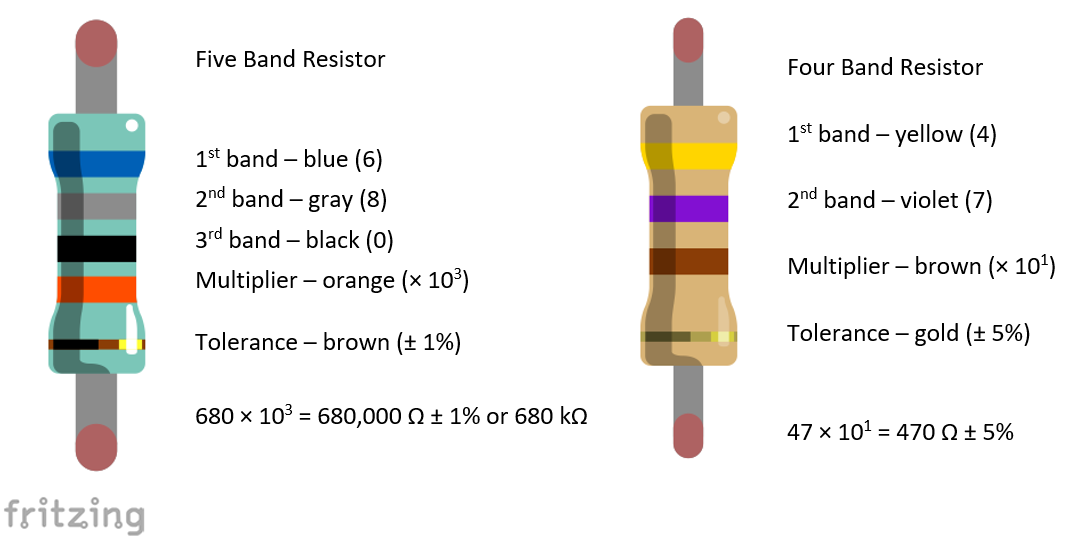
\includegraphics[width=12cm]{pics/resistor.png}
	\caption{Examples of a 5-band and 4-band resistor}
	\label{resistor}
\end{figure}





\end{document}




